\chapter{Office 和 WPS——办公样样行}
\label{cha:office-and-wps}

\begin{intro}
  让我们从最常见的办公软件——Office 和 WPS,来开始我们的软件篇旅程。在阅读完这一章后,你能找到下面这些问题的答案:
  \begin{itemize}
    \item Word、PowerPoint(简称 PPT)、Excel、Office、WPS 这几个词之间有什么关系?
    \item Office 版本好多,我该选哪个?2003?2007?2019?
    \item 为什么我电脑上自带的 Office 点开之后却打开了一个网页/购买链接?
    \item Office 怎么安装?为什么还要花钱购买?
    \item WPS 跟 Office 有什么区别?我如何在它们当中选择?
  \end{itemize}
\end{intro}

我们绝大多数人使用电脑,都逃不开「文档写作」「幻灯片制作」「表格处理」这么三件事。也许你早已会用 WPS,或者 Word、PowerPoint 以及 Excel 这些再熟悉不过的软件来做这三件事,但这些软件背后的故事或许并不为你所知晓。

需要强调的是,这部分并不是一份 Office 软件教程。我们不会介绍有关 Office 和 WPS 具体的使用方法——如果想要学习这些软件,不妨在看完本章后,按照\chapref{cha:how-to-find-tutorials}所介绍的方法去寻找 Office 的教程。

\section{Microsoft Office}

Microsoft Office 是由微软开发的办公软件套装。称它「软件套装」,是因为 Microsoft Office 是一系列软件的组合,而非单单一款软件。Microsoft Office 一般被人们直接简称为「Office」,包含了一系列面向办公领域的子软件:

\begin{itemize}
  \item \regcolor{Word,用于制作电子文稿;}
  \item \regcolor{PowerPoint(往往俗称「PPT」),用于制作幻灯片;}
  \item \regcolor{Excel,用于制作表格和进行数据处理;}
  \item OneNote,用于制作数字化的笔记,可以搭配触摸屏、手写笔和数位板等使用;
  \item Access,用于制作和管理数据库;
  \item Publisher,用于设计出版物;
  \item Visio,用于绘制流程图、示意图等图形;
  \item ……
\end{itemize}

上面列表中的前三位——Word、PowerPoint 和 Excel,是 Office 套装中人们耳熟能详的三个子软件,民间又俗称「Office 三件套」。它们三个能满足普通人大多数的基本办公需求,具有庞大的用户群体;相比之下,其他 Office 子软件的知名度就不那么高了,安装使用它们的人也相对不多。

目前(2024 年),最新版本的 Office 三件套的软件图标如下图所示。

\begin{figure}[htb!]
  \centering
  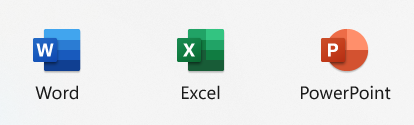
\includegraphics[width=.5\textwidth]{assets/software/Office_icons.png}
  \caption{如今的 Office 三件套图标}
  \label{fig:Office_icons}
\end{figure}
\vspace*{-1cm}

\subsection{Office 的历史与版本}

Office 是一款历史悠久的软件套装,它诞生于二十世纪八九十年代。传统上,Office 使用发行年份作为版本名称。让我们从 Office 2003 开始,看一看 Office 的「进化之路」。

Office 2003 是十分经典的一代 Office。与现在的 Office 软件界面有很大不同,Office 2003 的功能按钮是一排排罗列在软件界面上方的。下图是 Word 2003 的软件界面,在你的回忆中,是否有这样的画面呢?

\begin{figure}[htb!]
  \centering
  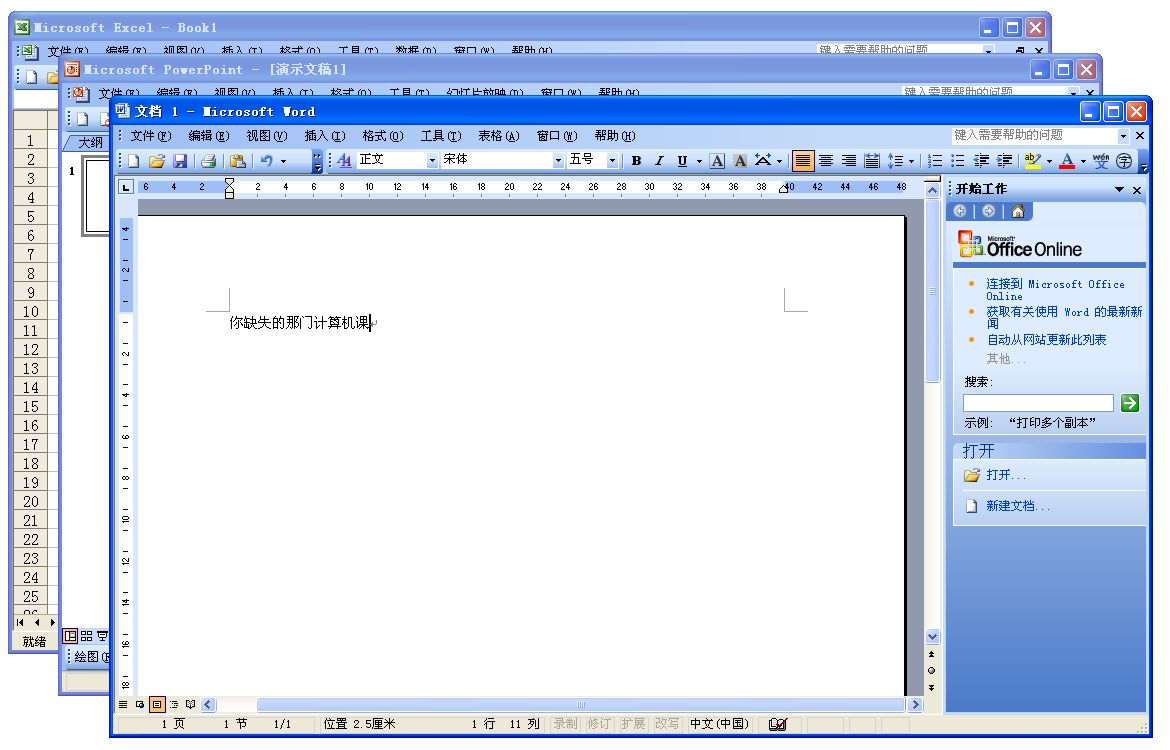
\includegraphics[width=.83\textwidth]{assets/software/Office_2003.png}
  \caption{Office 2003 的界面}
  \label{fig:Office_2003}
\end{figure}

经典归经典,但年代实在太过久远。如今的 2024 年,这一版「文物级」的 Office,除了部分尚未更新的中小学「信息技术」课堂等少见场景外,我们几乎很少再见到。

Office 2007 同样是经典的一代 Office。自这一代开始,Office 软件采用了一种新的用户界面,将各种各样的功能根据种类分列在不同的「标签卡」中,排列在界面上方。这种「大标签、大按钮」的结构称为「Ribbon」,如同\autoref{fig:Office_2007} 所示。此后,这一设计理念一脉相承,今天的 Office 的软件界面仍然有着 2007 版本的许多影子。

\begin{figure}[htb!]
  \centering
  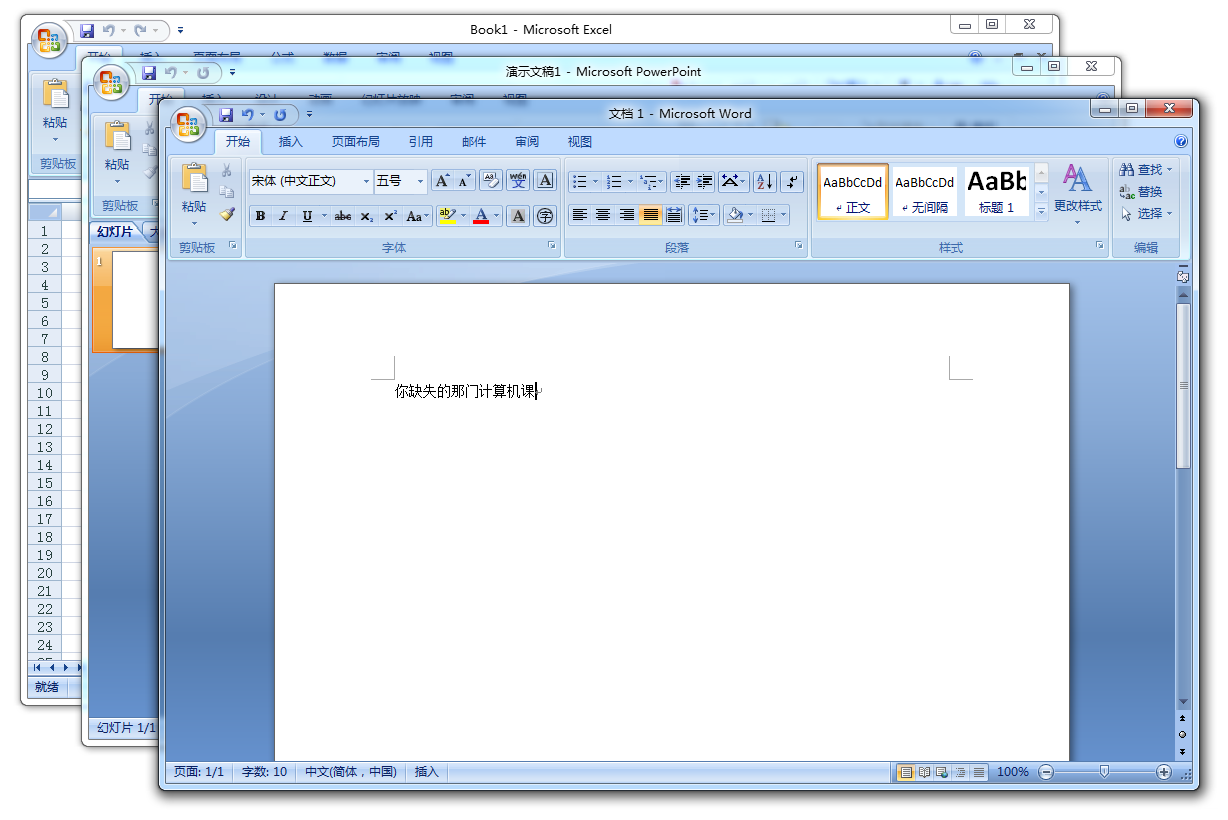
\includegraphics[width=.81\textwidth]{assets/software/Office_2007.png}
  \caption{Office 2007 的界面}
  \label{fig:Office_2007}
\end{figure}

但另一方面,这种新的界面与 2003 版及之前版本那种按钮一排排罗列的操作方式大相径庭。出于这个原因,当时许多人不愿意转向新版本,这也是 2003 成为「一代经典」的原因之一。

Office 2010 与 Office 2007 在软件界面和风格上并没有什么很大的差别。在 2021 年以前,我国计算机二级考试 Office 科目使用的就是 Office 2010 版本,下面的软件界面想必许多读者都不会陌生。

\begin{figure}[htb!]
  \centering
  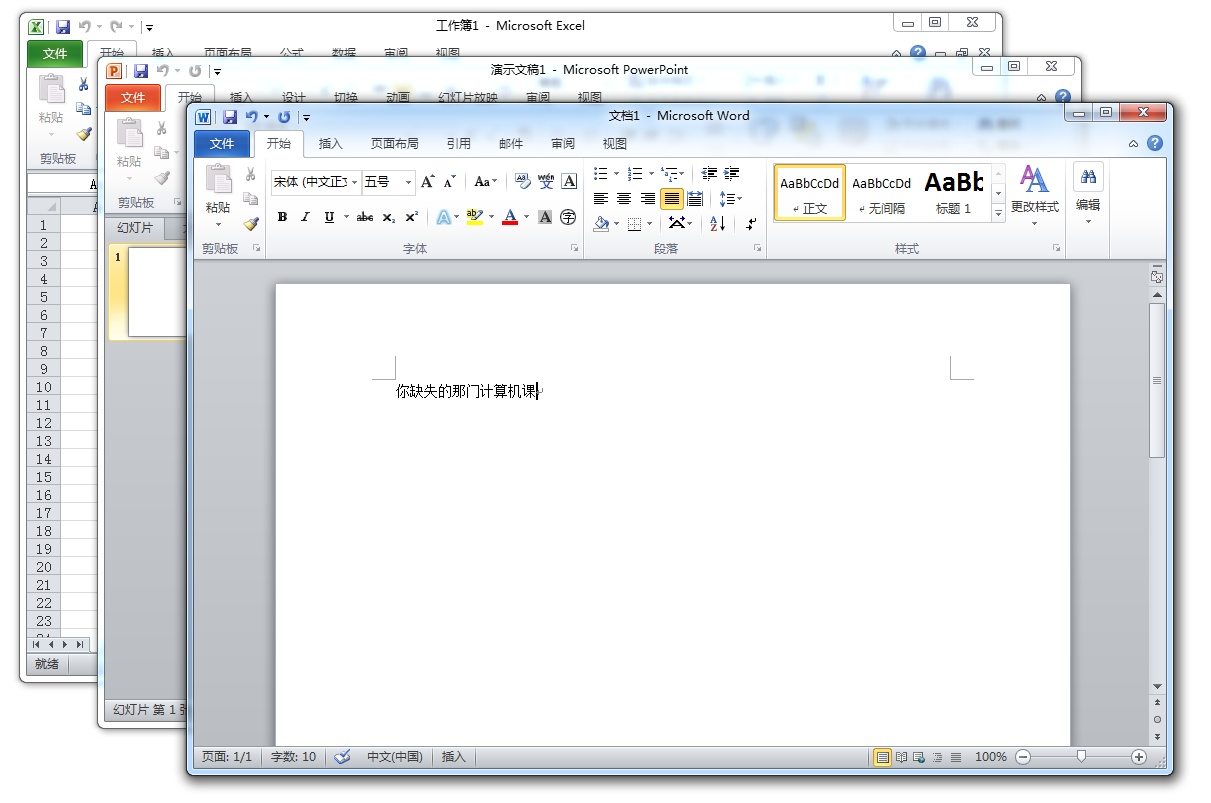
\includegraphics[width=.81\textwidth]{assets/software/Office_2010.png}
  \caption{Office 2010 的界面}
  \label{fig:Office_2010}
\end{figure}

自 Office 2013 开始,Office 的界面画风放弃了原来有些许立体感的「拟物」风格,转向了完完全全纯色块与简单几何图形构成的「扁平」风格,不过操作逻辑仍然继承了自 Office 2007 以来的那一套。不仅如此,后来将近十年内推出的版本——Office 2013、2016、2019 乃至 2021,都有着几乎相同的界面设计风格。\CJKsout*{(虽说「科技以换壳为本」,但这连壳都没怎么换。)}\autoref{fig:Office_2016} 是 Word 2016 的软件界面。

\begin{figure}[htb!]
  \centering
  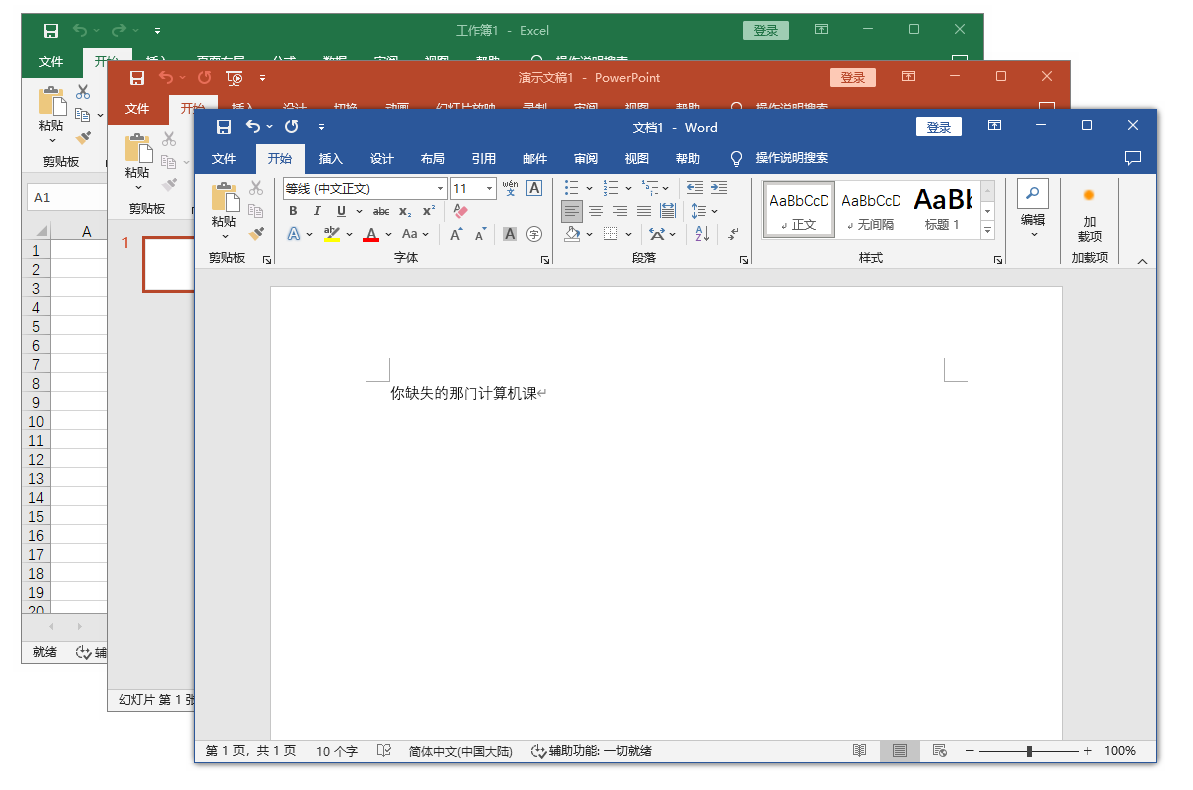
\includegraphics[width=.82\textwidth]{assets/software/Office_2016.png}
  \caption{Office 2016 的界面}
  \label{fig:Office_2016}
\end{figure}

而到了 2024 年,为了配合 Windows 11 的设计风格,微软在这一年的 Office 版本中稍稍更改了界面设计,采用了所谓「Fluent」的设计理念。虽然操作界面仍然沿用了 Ribbon 设计,但标题栏加高、加入搜索框,上方的 Ribbon 菜单也加入了圆角与阴影,给人以「立体浮动」的感觉。下图就是 Office 2024 的界面。

\begin{figure}[htb!]
  \centering
  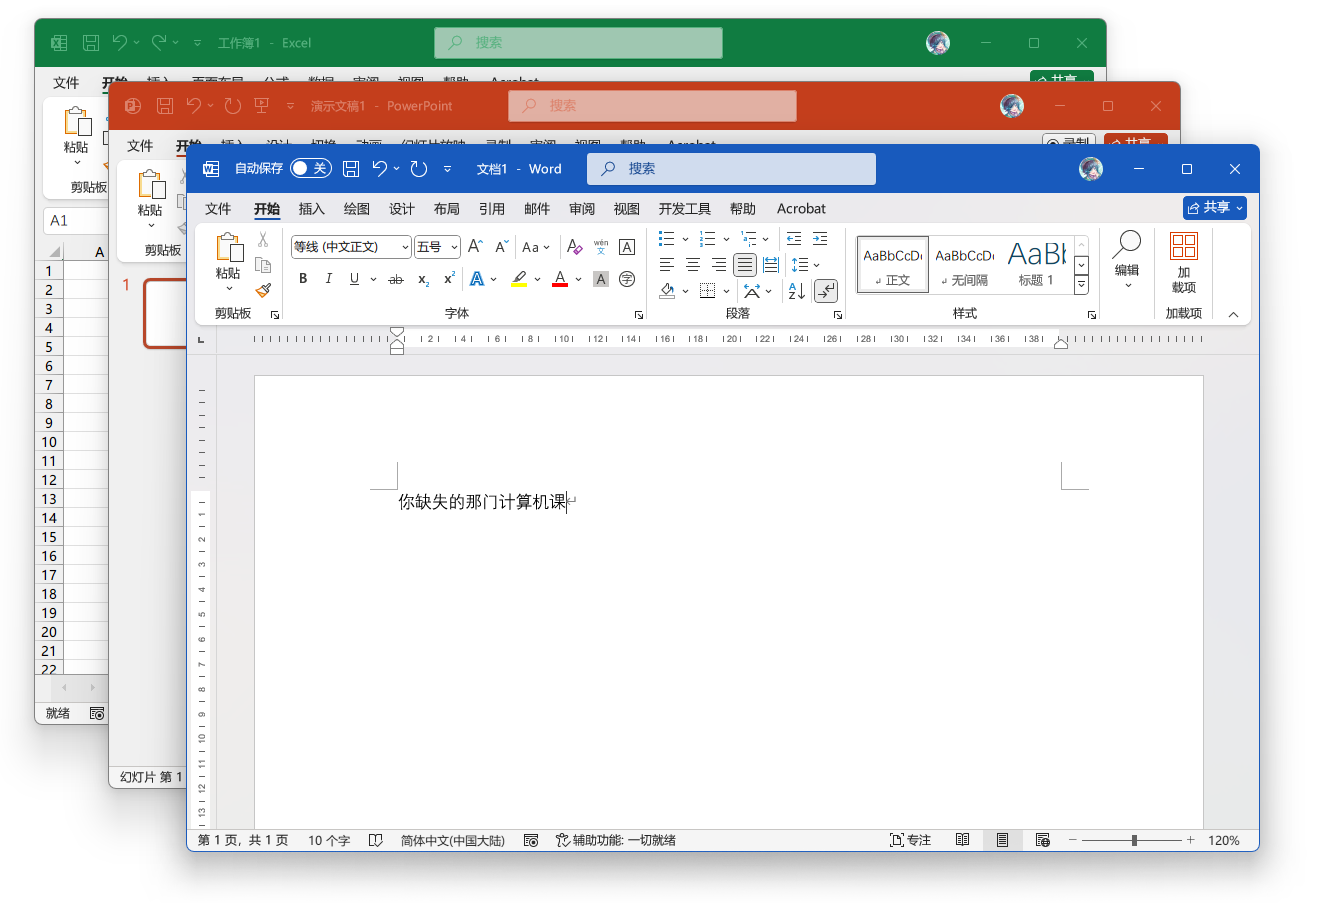
\includegraphics[width=.82\textwidth]{assets/software/Office_2024.png}
  \caption{Office 2024 的界面}
  \label{fig:Office_2024}
\end{figure}

在 Office 转向扁平风的那几年中,除了这种传统的「年份」Office,微软还推出了一种不断迭代更新的「Office 365」(现改名为「Microsoft 365」)。Office 365 采用持续「滚动更新」的策略,不再使用年份命名,这样始终能获得最新的功能。不过,事实上,Office 365 与年份版本 Office 的最大区别还是在于各项「云服务」,例如文件跨设备同步等。

\begin{note}
  自 2021 年开始,我国计算机二级考试 Office 科目使用了 Office 2016 作为考试软件。如上文所言,Office 2013--2021 乃至 Office 365 的软件界面和操作体验都没有明显的区别,故读者在练习时若实在没有 Office 2016,可以选用其余版本作为替代。
\end{note}

\subsection{Office 的文件格式}

在 Office 2003 及以前版本中,Office 三件套使用的文件格式的扩展名为 \MissingVerb{doc}、\MissingVerb{ppt} 和 \MissingVerb{xls}。而自 Office 2007 开始,微软推出了一套新的 Office 文件格式——「Office 开放 XML 格式」(Office Open XML,简称「OOXML」),对应的扩展名是 \MissingVerb{docx}、\MissingVerb{pptx} 和 \MissingVerb{xlsx},如下表所示。

\begin{table}[htb!]
  \centering
  \caption{不同的 Office 文件格式}
  \label{tab:office-formats}
  \begin{tblr}{
    colspec = ccc,
    row{1} = {valign=m, fg = white, bg = missing, font = \bfseries},
    row{even} = {MissingSkyBlue},
  }
    \toprule
    软件 & {旧格式扩展名\\(2003 及以前)} & {新格式扩展名\\(2007 及以后)} \\
    \midrule
    Word & \MissingTT{doc} & \MissingTT{docx} \\
    PowerPoint & \MissingTT{ppt} & \MissingTT{pptx} \\
    Excel & \MissingTT{xls} & \MissingTT{xlsx} \\
    \bottomrule
  \end{tblr}
\end{table}

尽管新格式看起来扩展名只是多了个字母 \MissingVerb{x},但是与旧版格式是\regcolor{完全不兼容}的。Office 2007 以及之后的各版本,可以打开新旧两种格式的文档,并且在保存文件时可以选择保存为新旧两种格式中的某一种。下图中,上方「Word 文档 (*.docx)」便是新格式,而下方「Word 97-2003 文档 (*.doc)」则是旧格式。

\begin{figure}[htb!]
  \centering
  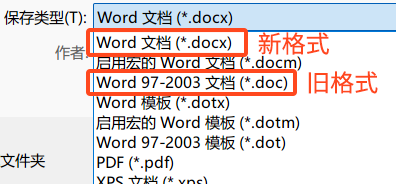
\includegraphics[width=.6\textwidth]{assets/software/Word_formats.png}
  \caption{Word 的保存选项}
  \label{fig:Word_formats}
\end{figure}

新格式(即扩展名带 \MissingVerb{x} 的那些格式)相比旧格式支持更多的功能和排版特性,自 Office 2007 以后的 Office 默认都保存为新格式。在今天人们普遍使用 Office 2007 及以上版本的情况下,我们建议始终为自己的文档选用新格式,除非你有明确的理由去选用旧格式,例如接收方指定了文件的扩展名。

\subsection{Office 的购买和安装}

Office 是付费软件。其中,Office 365 的付费方式是「订阅制」,每年都需要付费才能使用;而年份版本的 Office,则采用「买断制」,一次购买便可永久使用。同一版本的 Office(例如 Office 2019),又根据包含多少子软件、有无高级功能、售后服务等级等,分为不同的档次。例如「家庭与学生版」只包含 Word、PowerPoint 和 Excel 三件套,没有 VBA 等高级开发功能;「专业增强版」则包含几乎所有的 Office 功能,但售价高昂。下图是在微软官网购买 Office 365 的产品介绍页面。

\begin{figure}[htb!]
  \centering
  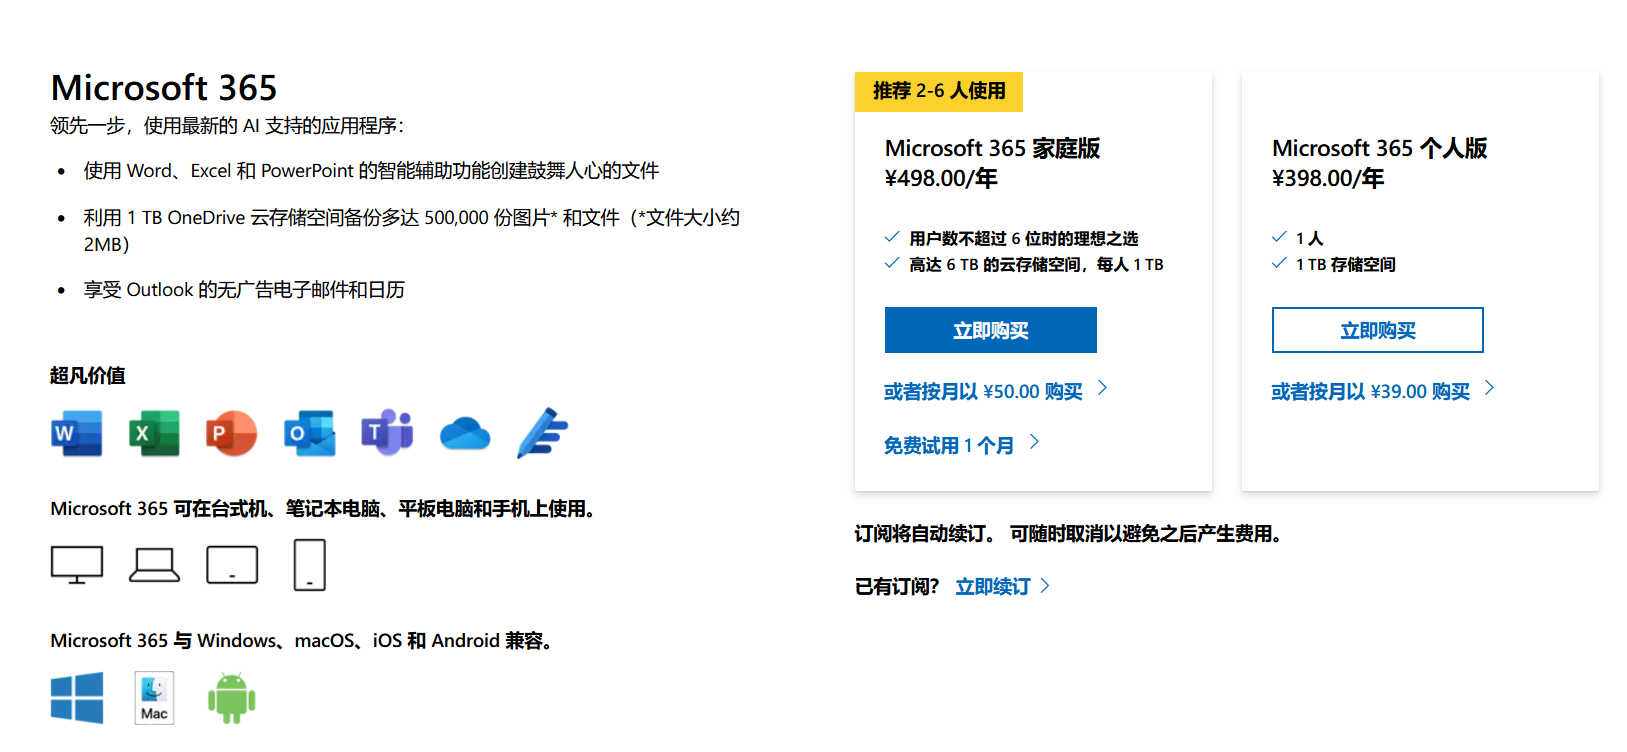
\includegraphics[width=.8\textwidth]{assets/software/Buying_Office_365.png}
  \caption{Office 365 了解一下}
  \label{fig:Buying_Office_365}
\end{figure}

如果需要购买 Office 365,可以前往\href{https://www.microsoft.com/zh-CN/microsoft-365/buy/microsoft-365}{微软官网}或者 Microsoft Store 购买。如果你是大学生或大学教职工,或许你所在的学校已经为你们批量购买过正版 Office 软件。此时,你可以通过查阅自己学校官网,或者咨询学校网络信息中心、正版软件服务中心等有关部门来了解正版 Office 的获取方式。下图是某学校正版软件平台的截图,在这里可以获取到正版的各版本 Office。

\begin{figure}[htb!]
  \centering
  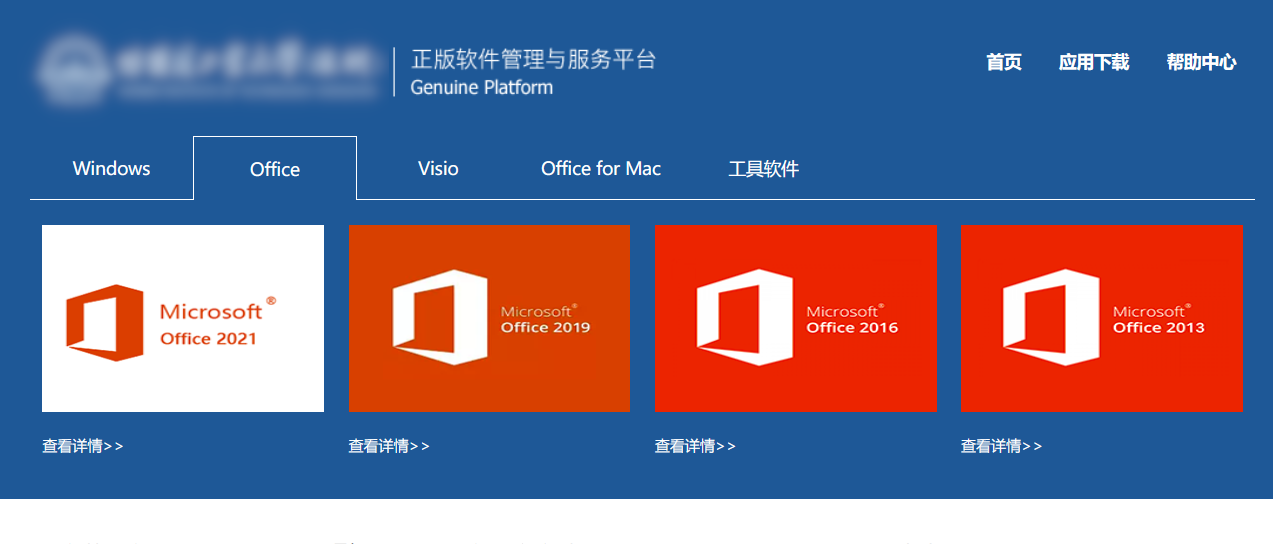
\includegraphics[width=.8\textwidth]{assets/software/Geniune_platform.png}
  \caption{某校提供的 Office}
  \label{fig:Geniune_platform}
\end{figure}

\begin{figure}[tb!]
  \centering
  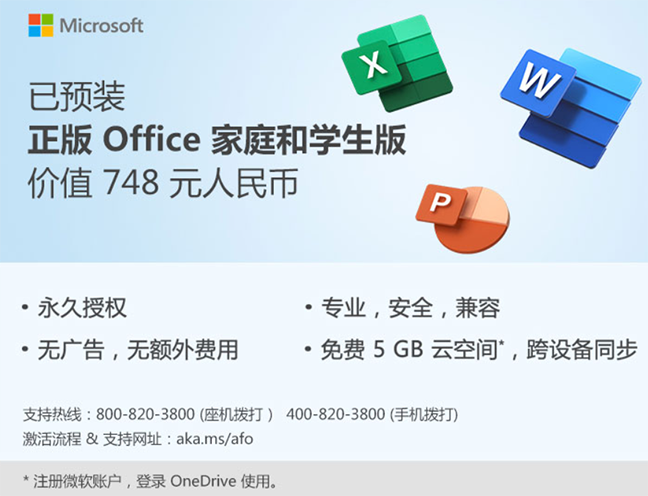
\includegraphics[width=.5\textwidth]{assets/software/Preinstalled_Office.png}
  \caption{买电脑送 Office}
  \label{fig:Preinstalled_Office}
\end{figure}

今天,许多笔记本电脑和品牌机台式机在出厂时会附赠用户一套正版 Office 软件。这种情况下,机器首次开机后就能看到内置的 Office 软件(通常包含 Word、PowerPoint 和 Excel)。我们只需要启动它们,按照软件的提示,登录或创建一个自己的微软账号,即可完成正版验证。不过,如果你是在电脑城组装的电脑,或者使用的非品牌零售渠道的机器,那么很可能没有这项福利。\autoref{fig:Preinstalled_Office} 是在电商平台购买某笔记本电脑时的 Office 附赠提示。

Office 软件的安装方式比较简单。取决于你获取到软件的方式,如果你是通过 Microsoft Store 购买的 Office,那么直接在 Microsoft Store 点击【安装】就可以完全搞定。对于通过其他官方途径获取的 Office 安装器,大多数情况下也只需要简单双击并按提示操作即可完成安装。

Office 这种软件自然免不了被盗版的命运。但是除了常规的盗版之外,在互联网还上有很多民间二次打包的「优化版」「精简版」「修改版」Office,它们在直接安装后,无需更多操作就能免费使用。我们非常不建议大家使用这些二次打包 Office——除了「盗版」本身不值得提倡外,这些二次打包的 Office 往往经过一些「魔改」,可能导致少数情况下软件工作不正常甚至无法使用。此外,这些魔改 Office 往往会有一些使用上的不便,例如每次启动时触发 UAC 弹窗(弹出窗口「你要允许此应用……」),以及文件关联莫名失效等。更有甚者,某些来历不明的 Office 软件很可能含有各种各样的病毒。下图是当我们试图在某网站上下载一个「Office 2007 三合一精简版」时,杀毒软件「卡巴斯基」弹出的提示。

\begin{figure}[htb!]
  \centering
  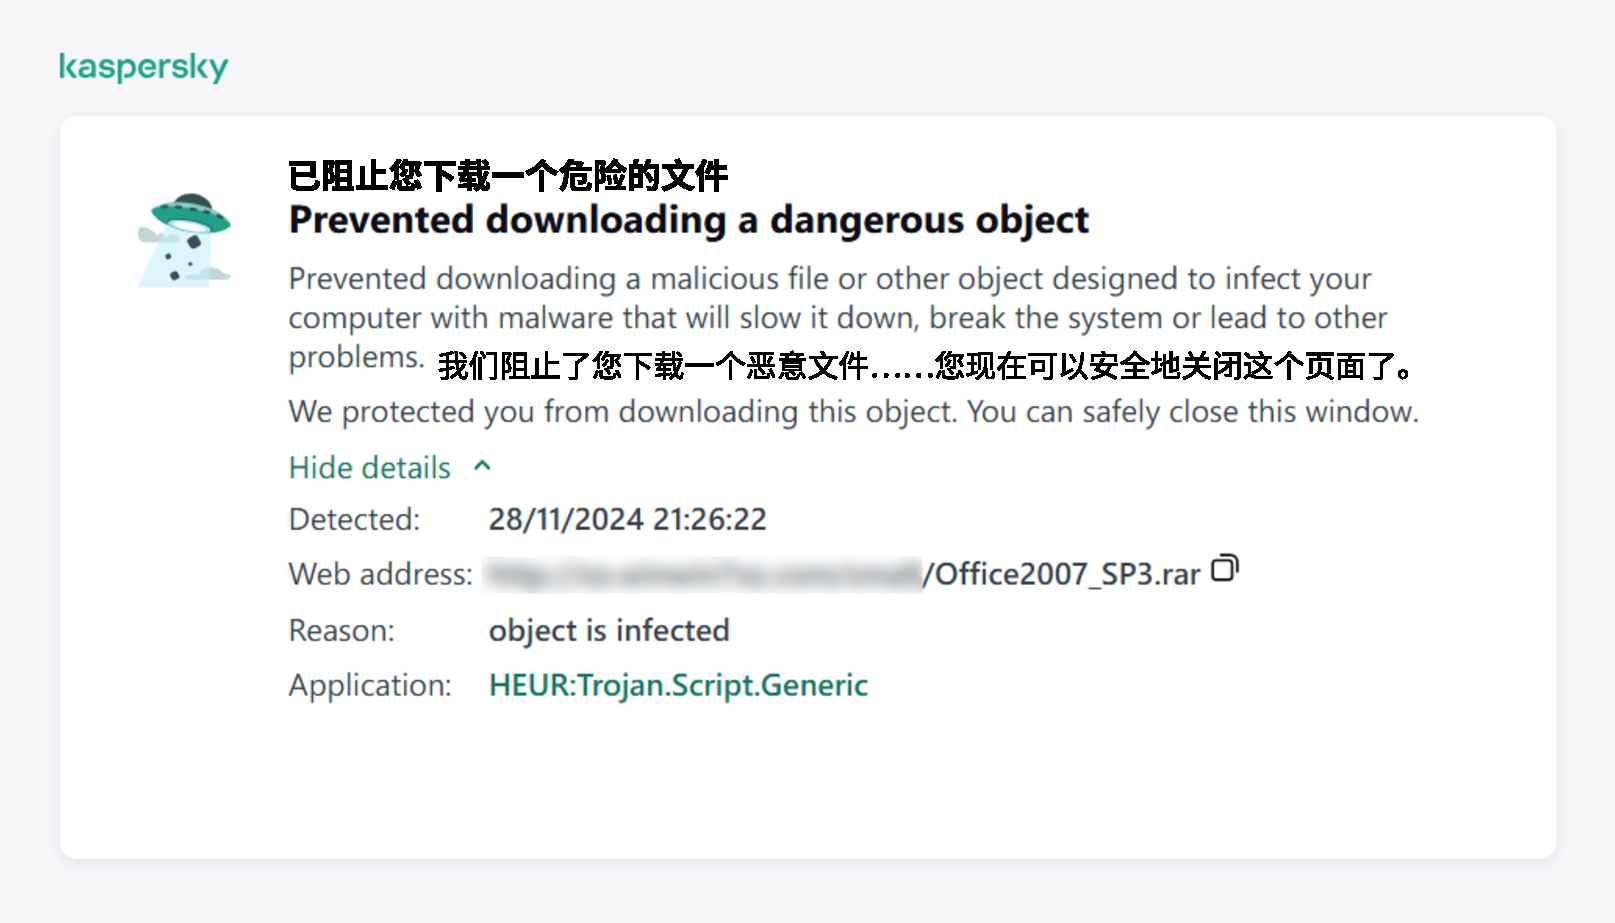
\includegraphics[width=.8\textwidth]{assets/software/Kaspersky_blocks_pirate_Office.pdf}
  \caption{卡巴斯基对「精简版」Office 的提示}
  \label{fig:Kaspersky_blocks_pirate_Office}
\end{figure}

\subsection{「网页版」 Office}

\begin{wrapfigure}[10]{r}{4cm}
  \centering
  \vspace*{3ex}
  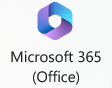
\includegraphics[width=3.5cm]{assets/software/Fake_Office.png}
  \caption{网页版Office的图标}
  \label{fig:Fake_Office}
\end{wrapfigure}

即使你没有购买和安装过 Office,你或许仍会发现电脑的「开始菜单」中有 Office 甚至 Word、PowerPoint、Excel 等软件的图标,又或者是一个叫「Microsoft 365 (Office)」的玩意,如右侧所示。如果你尝试去点击这些 app,会发现打开了一个网页。在这个页面按提示登录微软账号,最后会来到\autoref{fig:Fake_Office_2} 类似的页面。

这是微软提供的免费的「网页版」Office,类似于腾讯文档或金山文档等网页产品。点击左侧的 Word、Excel 等图标,会打开对应的网页版应用。它们可以免费使用,但只有相当基础的编辑功能,且只有在网络良好时才能正常工作,故只能作为没有安装 Office 的应急替代品。

这个「网页版」Office 本质就是几个链接,没有软件的本体,但也可以卸载。卸载方式参见\chapref{cha:basic-maintenance}。

\begin{figure}[htb!]
  \centering
  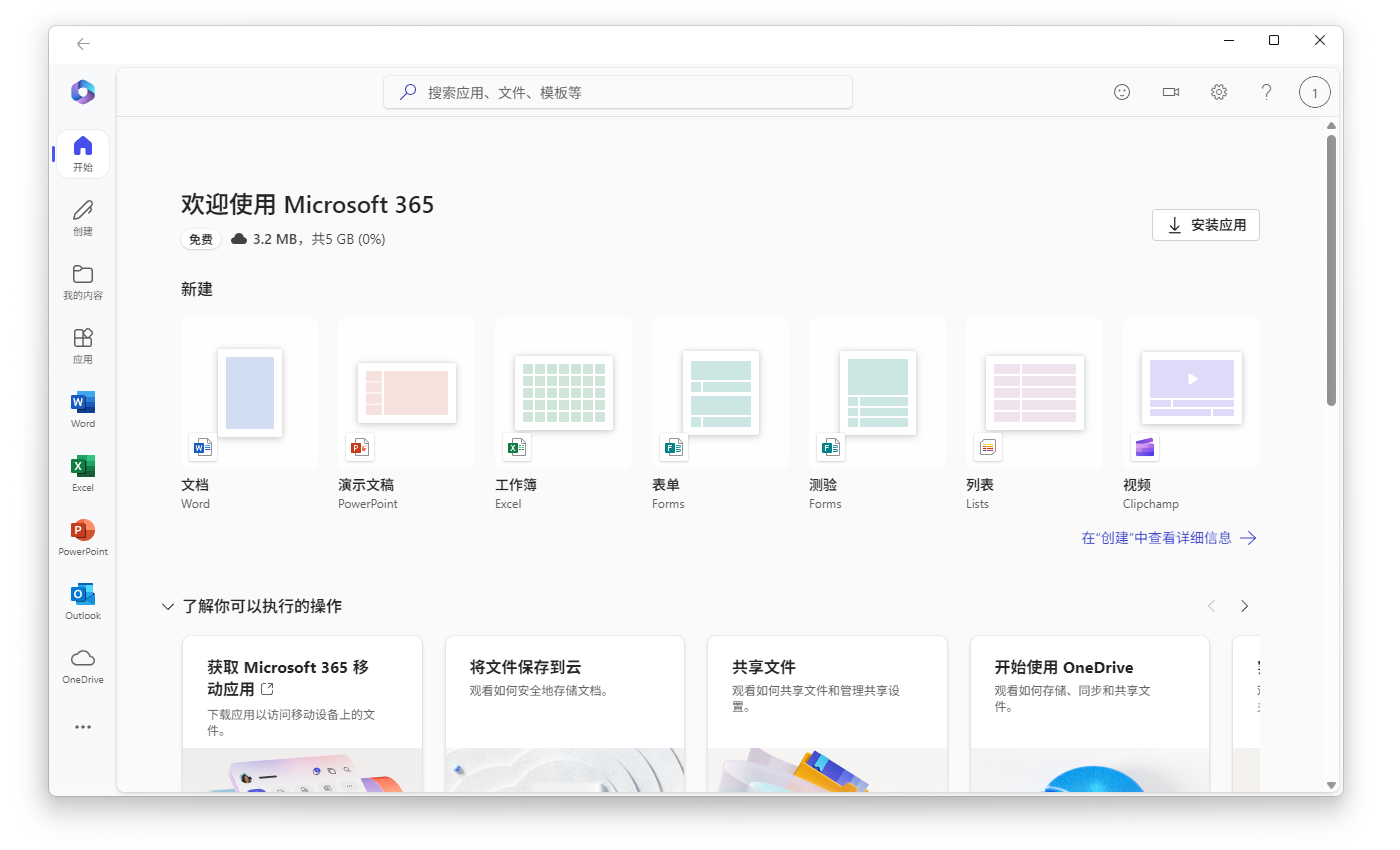
\includegraphics[width=.7\textwidth]{assets/software/Fake_Office_2.png}
  \caption{网页版Office的界面}
  \label{fig:Fake_Office_2}
\end{figure}

\subsection{选择 Office 的原因}

在今天,Office 文件格式(即 \MissingVerb{doc}、\MissingVerb{pptx} 等文件格式)在人们的日常工作中有着绝对无可动摇的地位——绝大多数的工作资料都是通过这套格式的文件进行交换的。Office 作为推出这套格式的本家,自然与这套格式最为契合。因此,\regcolor{选择 Office 的最主要原因,便是它对 Office 文件格式的无缝支持}。WPS 尽管对这套格式也有着相当高的支持度,但在少数情况下,仍然会出现排版错乱、内容丢失等情况。至于其他办公软件,大多对于 Office 文件格式的支持只能说「勉强」。

选择 Office 的另一个原因是,\regcolor{Office 作为微软自家出品的软件,在 Windows 操作系统上具有相对出色的性能表现和操作体验}。在一众办公软件中,Office 的操作手感比较舒适,且与 WPS 相比,Office 界面简洁、没有繁杂的广告和其他多余功能。

\section{WPS Office}

\regcolor{WPS Office 是除了微软 Office 自身外,对 Office 文件格式(包含新旧两种格式)支持最好的办公软件},可以说没有之一。人们一般会把 WPS Office 简称为「\regcolor{WPS}」,它包含三个主要的子组件,分别是「WPS 文字」「WPS 演示」和「WPS 表格」,依次对标 Office 套装中的 Word、PowerPoint 和 Excel。WPS 使用类似于 Office 的界面,默认使用 Office 文件格式进行文件保存,因而在大多数情况下都可以作为 Office 的替代品。

\subsection{WPS 的历史}

\begin{figure}[htb!]
  \centering
  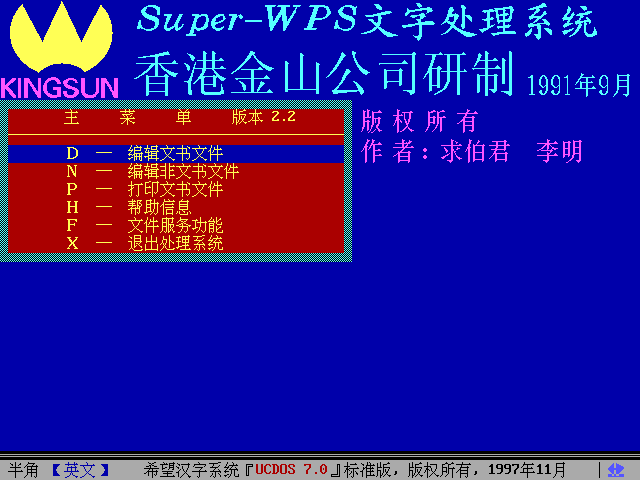
\includegraphics[width=.5\textwidth]{assets/software/Super-WPS.png}
  \caption{Super-WPS 的界面}
  \label{fig:Super-WPS}
\end{figure}

WPS 是由我国公司金山软件开发的免费软件,但与很多人的臆想不同,WPS 并不是靠模仿 Office 起家的。1989 年,来自金山的年轻工程师求伯君开发了一款中文文字处理系统(word processing system,简称 WPS),名叫「Super-WPS」,一经出现,风靡全国,几乎占据了中国文字处理软件市场的绝大部分份额。\autoref{fig:Super-WPS} 是 Super-WPS 的启动界面。

但彼时的 Super-WPS,运行在 DOS 系统上(就是那个「漆黑的屏幕上闪烁着 \MissingVerb{C:>_}」的操作系统),所以使用起来并没有今天的 WPS Office 这般方便与所见即所得(What you see is what you get,简称 WYSIWYG)。在编辑状态下,你没有办法看到文本真正在纸上呈现的样子,要想知道效果,必须切换到「打印预览」模式,而这个模式又无法直接编辑内容。不过,虽然麻烦,但比一无所有还是好上许多。\autoref{fig:Super-WPS_Editing} 左侧是编辑模式,右侧则是「打印预览」模式。

\begin{figure}[htb!]
  \centering
  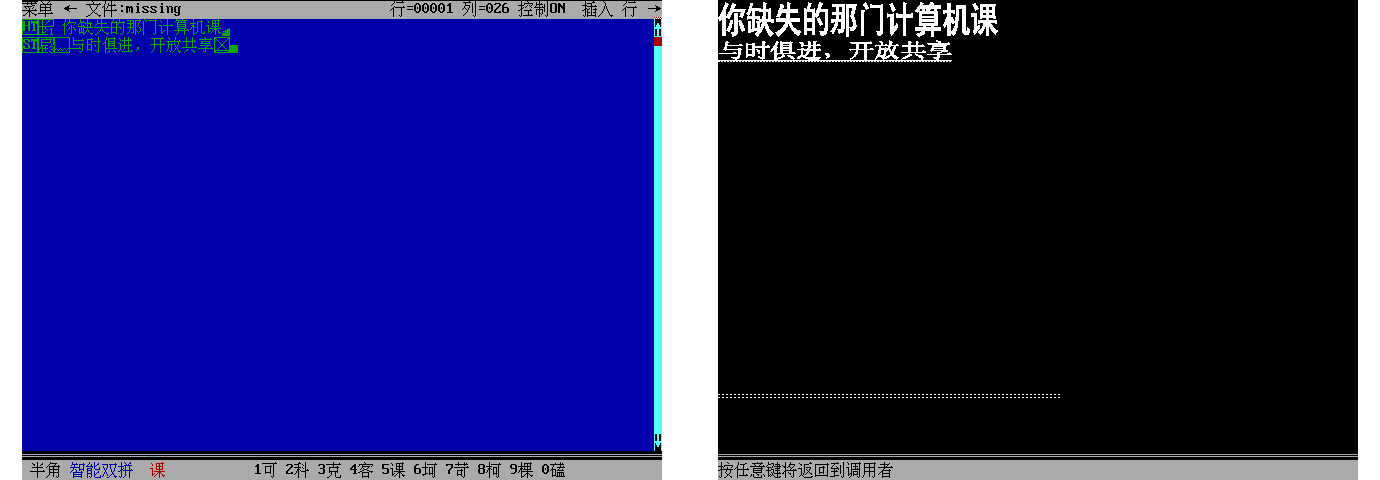
\includegraphics[width=.98\textwidth]{assets/software/Super-WPS_Editing.png}
  \caption{Super-WPS 的编辑模式(左)与打印预览(右)}
  \label{fig:Super-WPS_Editing}
\end{figure}

1990年,微软发布了首个面向 Windows 平台的 Office 版本。然而,由于当时 Office 对中文的支持不够完善,而市场早已习惯使用 Super-WPS,Office 在中国并未引起太大的反响。1996 年,为了能在中国市场分一杯羹,微软与金山达成了共享协议,使双方可以交叉使用彼此的文件格式。这一协议让 WPS 得以兼容 Office 文件,但也让微软凭借其庞大的体量优势以及对盗版的放任态度,迅速占领了中国文字处理软件的绝大部分市场。自此,WPS 在激烈的竞争中逐渐失去了市场主导地位。

为了应对这一局面,WPS 开始向微软的 Office 学习,从最初的单一「文字处理系统」发展为与 Office 类似的综合办公软件套装,并在操作界面上向 Office 靠拢,以提升用户的使用习惯与兼容性。如今,WPS 已不仅仅是一款办公软件,更融入了「协作办公」「云服务」等多项增值功能,逐步构建起了一套完整的办公解决方案体系,在竞争中重新找到了自己的定位与市场机会。

\subsection{选择和不选择 WPS 的理由}

WPS 对 Office 文件格式有着高度的兼容性,这意味着在绝大多数情况下 WPS 都可以作为 Office 软件的替代品。而 WPS 的界面与同时代 Office 软件的界面高度相似,下图是 2024 年末最新版本的 WPS 的截图。所以,对于大多数 Office 软件中的操作,WPS 中的操作方式都是相同或近似的。此外,WPS 是免费软件。这意味着,你可以在没有任何额外成本的情况下合理合法地使用它\footnote{严格来说,我们通常下载的「WPS」实际上是「WPS 软件个人版」。根据其最终用户许可协议,该版本仅限于个人计算机上使用。},同时获得对 Office 文件格式的最大兼容度并保持 Office 的使用习惯。

\begin{figure}[htb!]
  \centering
  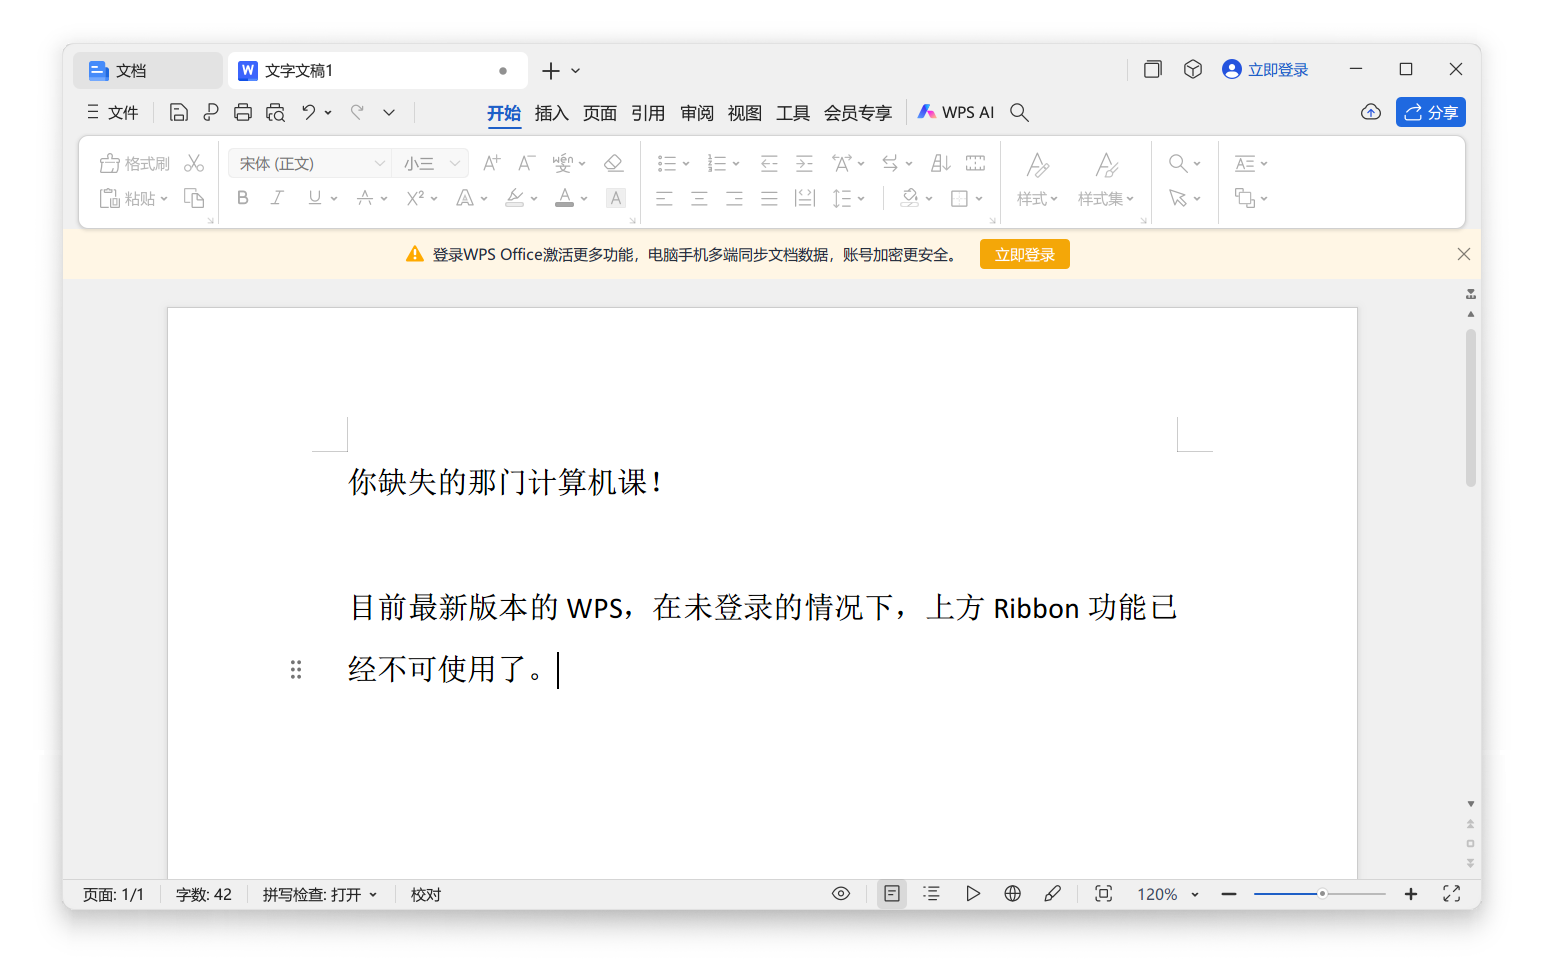
\includegraphics[width=.8\textwidth]{assets/software/WPS_Office.png}
  \caption{WPS 的界面}
  \label{fig:WPS_Office}
\end{figure}

WPS 针对中国用户的使用习惯推出了一系列额外功能。例如,WPS 有一套自己的模板库。在其中,你能找到各种各样的适合不同场景的文稿、幻灯片和表格模板,并将它们应用在自己的文档之中(可能需要额外付费)。在一些情况下,使用这些模板能够省时省力地制作出精美的文档。又比如,WPS 提供了自己的云服务平台(金山文档),借助金山文档能够实现多人协同编辑文件等高级功能。下图是 WPS 提供的部分模板。

\begin{figure}[htb!]
  \centering
  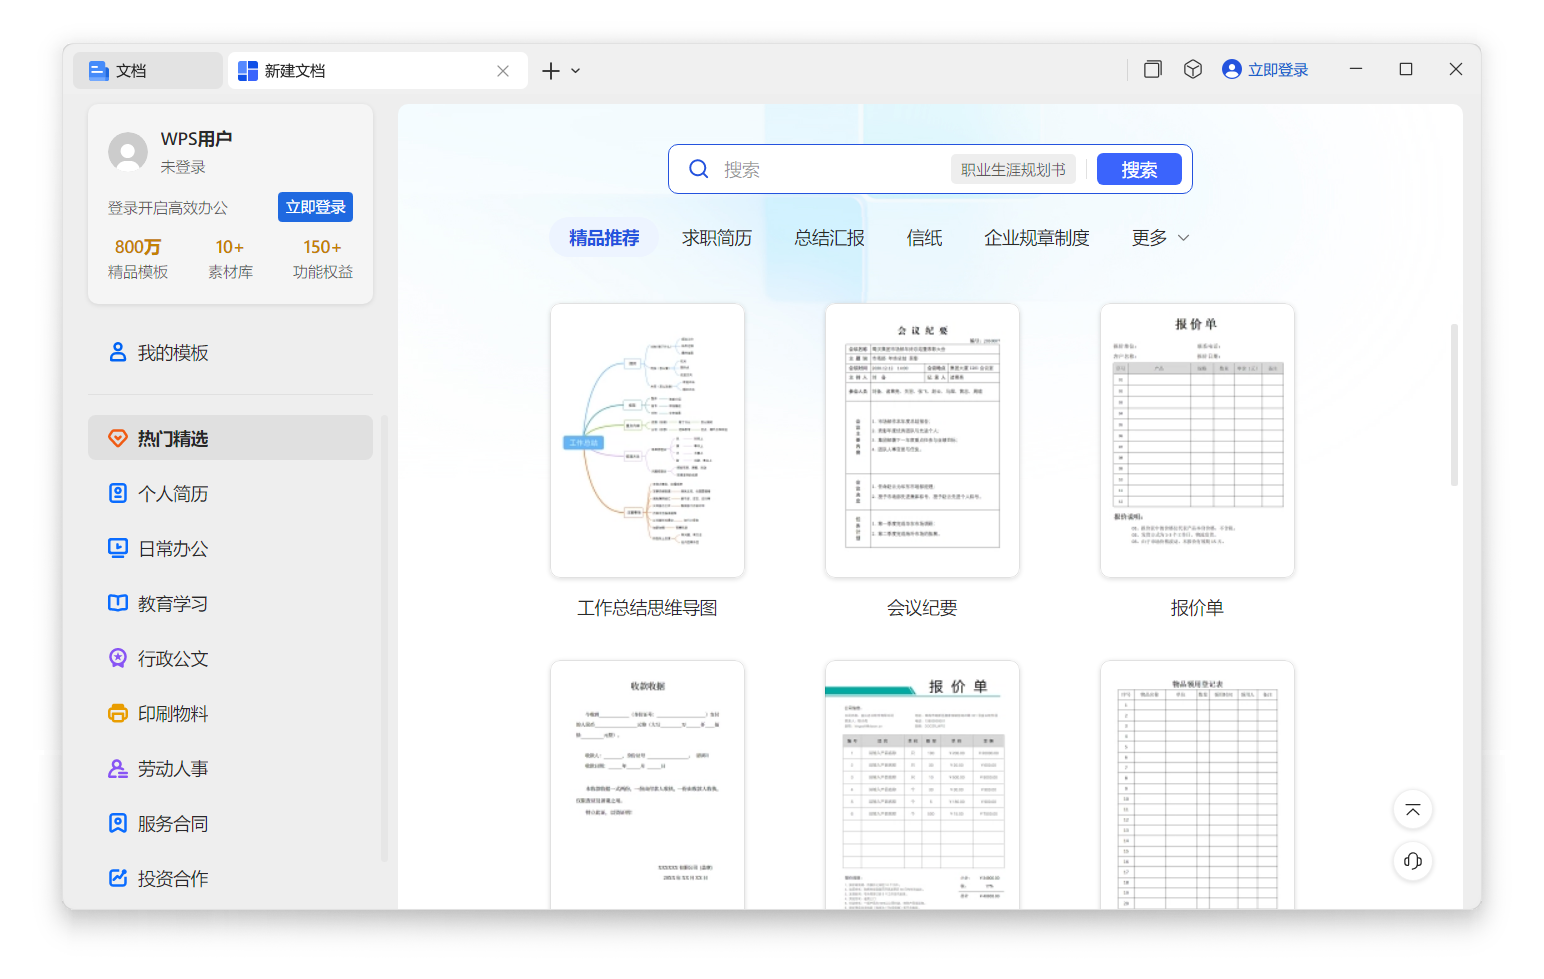
\includegraphics[width=.8\textwidth]{assets/software/WPS_templates.png}
  \caption{WPS 提供的模板}
  \label{fig:WPS_templates}
\end{figure}

然而,作为国产软件的 WPS,自然有着一系列国产软件常有的问题——例如,一些广告和「不登录不给用」。在上一小节的 WPS 主界面截图中,可以看到整个 Ribbon 区域的按钮都呈灰色状态,下方还有显眼的登录提示。只有在注册并登录一个金山办公账号之后,才能使用完整的应用功能。对于那些注重数据私密性的用户来说,这无疑是一个极大的缺点。

\begin{figure}[htb!]
  \centering
  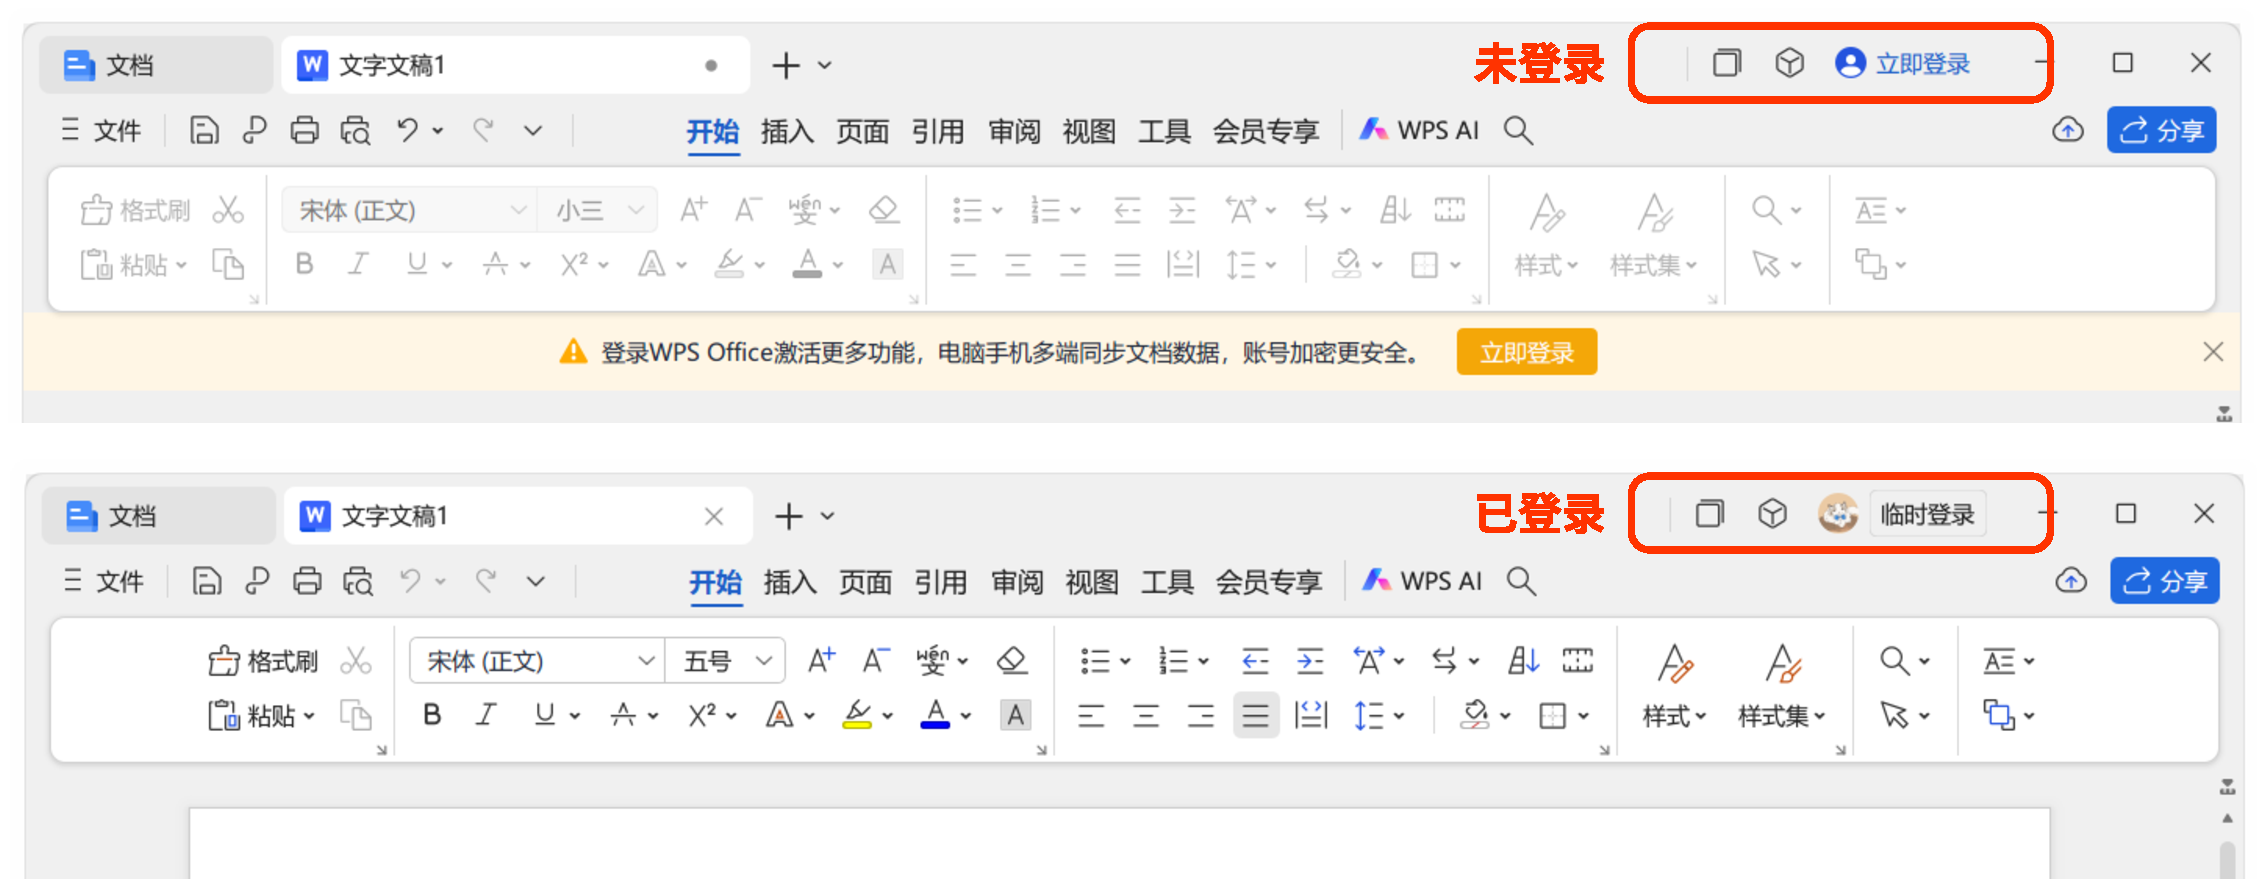
\includegraphics[width=.8\textwidth]{assets/software/WPS_no_login.pdf}
  \caption{只有登录才能用}
  \label{fig:WPS_no_login}
\end{figure}

\practice

\begin{enumerate}
  \item 你电脑上安装有 Office 吗?你能熟练地使用它们吗?你知道你所使用的 Office 软件的版本吗?
  \item 你有使用过 WPS 吗?如果有,试试探索它提供的各种模板。
  \item 前往电商平台查看一些笔记本电脑的商品详情,看看它们是否有将正版 Office 软件一并附赠。
\end{enumerate}